%%%%%%%%%%%%%%%%%%%%%%%%%%%%%%%%%%%%%%%%%%%%%%%%%%%%%%%%%%%%%%%%%%%%%%%%
%                                                                      %
% This program is free software; you can redistribute it and/or modify %
% it under the terms of the GNU General Public License as published by %
% the Free Software Foundation; either version 2 of the License, or    %
% (at your option) any later version.                                  %
%                                                                      %
% This program is distributed in the hope that it will be useful,      %
% but WITHOUT ANY WARRANTY; without even the implied warranty of       %
% MERCHANTABILITY or FITNESS FOR A PARTICULAR PURPOSE.  See the        %
% GNU General Public License for more details.                         %
%                                                                      %
% You should have received a copy of the GNU General Public License    %
% along with this program; if not, write to the Free Software          %
% Foundation, Inc., 51 Franklin St, Fifth Floor, Boston,               %
% MA  02110-1301  USA                                                  %
%                                                                      %
%%%%%%%%%%%%%%%%%%%%%%%%%%%%%%%%%%%%%%%%%%%%%%%%%%%%%%%%%%%%%%%%%%%%%%%%
%
%	$Id$
%
\setcounter{remarque-cnt}{1}
\setcounter{example-cnt}{1}
\chapter{Concepts de base sous {\Unix}}
\thispagestyle{fancy}

%%%%%%%%%%%%%%%%%%%%%%%%%%%%%%%%%%%%%%%%%%%%%%%%%%%%%%%%%%%%%%%%
\section{Notions g{\'e}n{\'e}rales}

{\Unix} est un syst{\`e}me d'exploitation orient{\'e} fichiers contrairement
{\`a} {\DOS}\footnote{{\DOS}= Microsoft Disk Operating System} ou {\`a}
{\OpenVMS}\footnote{VMS = Virtual Memory System, syst{\`e}me de Digital Equipment}
qui sont plut{\^o}t orient{\'e}s disque. Il n'existe pas sous {\Unix}, au
niveau utilisateur, de notion de disques physiques. On ne voit qu'une
seule arborescence dont diff{\'e}rents points sont rattach{\'e}s {\`a} un syst{\`e}me de
fichiers. Celui-ci peut correspondre physiquement {\`a}~:
\begin{itemize}
	\item une partition d'un disque physique (la partition peut correspondre
	      soit {\`a} une partie ou bien {\`a} la totalit{\'e} d'un disque physique)~;
	\item un ensemble de disques physiques, notion qu'il est possible d'utiliser soit dans
un environnement RAID~1, soit {\`a} partir d'un volume logique ({\sl Logical Volume})
dans l'environnement LVM\footnote{LVM: Logical Volume Manager. Cet outil, d{\'e}velopp{\'e}
{\`a} la base par IBM pour ses syst{\`e}mes AIX est pr{\'e}sent maintenant sur la plupart
des {\Unix} commerciaux et dans les environnements {\Linux}.}, soit un
{\sl Meta Device} sous Sun Solaris~;
	\item un syst{\`e}me de fichier distant r{\'e}sidant sur une autre machine du r{\'e}seau
	      (service NFS entre machines {\Unix}, ou service SMB/CIFS avec l'environnement {\Windows}).
\end{itemize}

La figure \ref{fig-bcpts-orgdisk} donne un aper\c{c}u des liaisons possibles
entre certains points de l'arborescence et les disques physiques sur une
machine {\Unix}.

\begin{figure}[hbtp]
\centering
	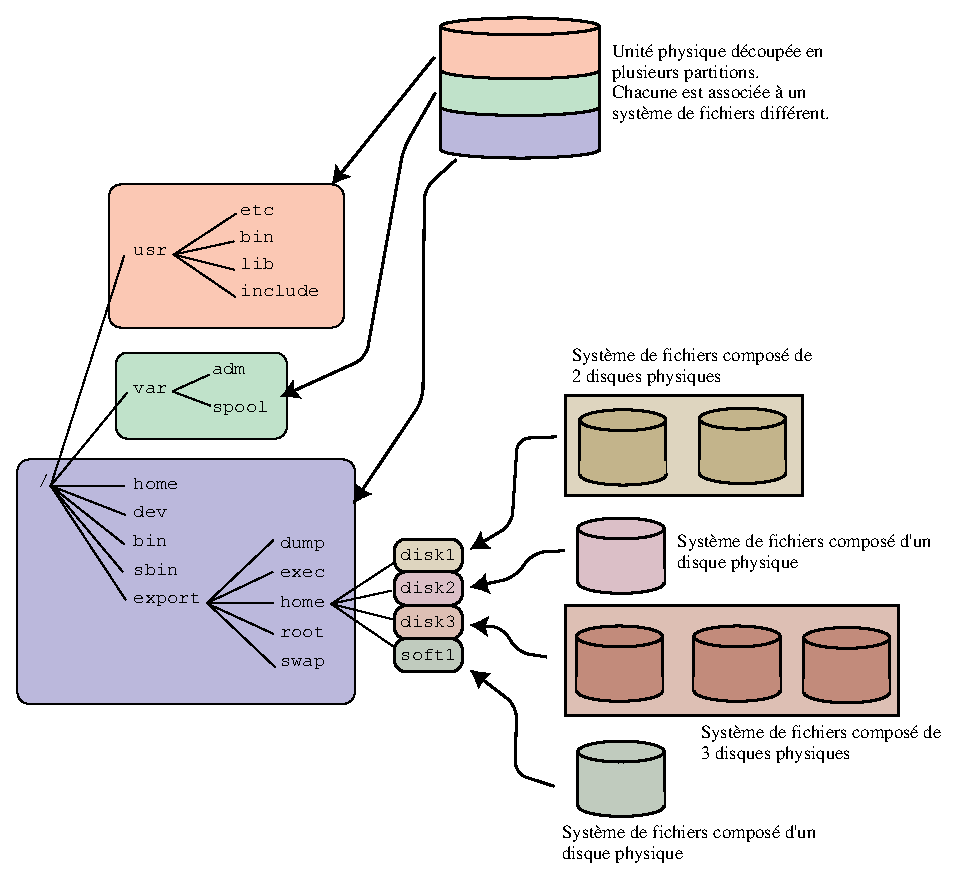
\includegraphics{base-concepts/orgdisk}[l]
	\caption{\label{fig-bcpts-orgdisk}Organisation de l'arborescence {\Unix} avec les syst{\`e}mes de fichiers}
\end{figure}

Toutes les commandes {\Unix} distinguent les majuscules des
minuscules. Par exemple <<~{\tt ls}~>>, <<~{\tt Ls}~>> , <<~{\tt lS}~>>
et <<~{\tt LS}~>> sont quatre mots diff{\'e}rents au niveau de
l'interpr{\'e}teur de commandes.

Chaque commande {\Unix} est ex{\'e}cut{\'e}e dans un process
s{\'e}par{\'e}. Lorsqu'on tape une commande au niveau de
l'interpr{\'e}teur de commandes, celui-ci cr{\'e}e un sous processus dans
lequel il ex{\'e}cute la commande. Lorsque celle-ci est termin{\'e}e, le
sous process disparait en rendant la main au processus p{\`e}re.

%%%%%%%%%%%%%%%%%%%%%%%%%%%%%%%%%%%%%%%%%%%%%%%%%%%%%%%%%%%%%%%%%%%%%
\section{\label{bcpts-login}Connexion et d{\'e}connexion}

Comme tout syst{\`e}me multi-utilisateurs et multi-t{\^a}ches, {\Unix} associe
{\`a} chaque utilisateur~:
\begin{itemize}
	\item	un nom appel{\'e} \index{login@\textsl{login}}<<~{\sl login}~>>
			({\'e}quivalent au <<~{\sl Username}~>>.
			de {\OpenVMS}, ou au <<~{\sl logon name}~>> de {\WindowsNT})~;
	\item	un mot de passe~;
	\item	un num{\'e}ro d'utilisateur unique ou \index{UID}
			<<~{\sl UID}\footnote{{\sl UID}~=~User IDentifier}~>> ({\'e}quivalent
			{\`a} l'<<~{\sl UIC}~>> {\OpenVMS} ou <<~{\sl logon ID}~>> de
			{\WindowsNT}).
\end{itemize}

Par cons{\'e}quent, la premi{\`e}re chose que vous demandera le syst{\`e}me sera
votre <<~{\sl login}~>> et votre mot de passe. Si les deux sont valides,
{\Unix} initialisera votre environnement de travail.

\begin{remarque}
Pour des raisons de s{\'e}curit{\'e}, comme sous {\OpenVMS} et
{\WindowsNT}, {\Unix} ne verifie pas que le nom de <<~{\sl login}~>>
existe. Une fois que les deux informations seront saisies,
c'est-{\`a}-dire nom de <<~{\sl login}~>> et mot de passe, il ira
chercher dans la base des utilisateurs s'il existe un enregistrement et
un seul pour lesquelles ces deux informations sont exactes. Si cela,
n'est pas le cas, {\Unix} affichera le message d'erreur suivant~:
\begin{center}
\begin{verbatim}
Invalid login name.
\end{verbatim}
\end{center}
sans autre forme de renseignements.
\end{remarque}

En fonction du type de poste de travail, c'est-{\`a}-dire terminal passif ou
station de travail disposant d'un environnement graphique, la m{\'e}thode de
d{\'e}con\-nexion du syst{\`e}me varie.

Si votre environnement de travail est sur un terminal passif, la commande
de d{\'e}connexion est~:
\begin{quote}
\index{exit@\texttt{exit}}{\tt exit}
\end{quote}

Dans le cas des stations de travail graphiques, cela d{\'e}pend de l'interface
s{\'e}lectionn{\'e}e. En effet, il en existe plusieurs types dont~:
\begin{itemize}
	\item	<<~{\sl CDE}~>> ou <<~Common Desktop Environment~>>, environnement
			graphique d{\'e}velopp{\'e} {\`a} la base sur les stations Hewlett-Packard
			({\sl HP--VUE}) et r{\'e}pandue sur l'ensemble des {\Unix}s commerciaux
			comme {\sl Solaris}, {\sl Digital {\Unix}}, {\sf HP--UX},
			{\sf AIX}, {\sl Irix}, etc.
	\item	<<~{\sl fvwm95}~>>, environnement r{\'e}git par la <<~{\sl Free Software
			Foundation}~>> livr{\'e} de base avec {\Linux}, environnement
			dont la pr{\'e}sentation ressemble {\`a} {\Windows}95 (et sup{\'e}rieur)
			et {\WindowsNT} 4 (ou sup{\'e}rieur). Les sources de cet environnement
			sont disponibles et libres d'acc{\`e}s. Il est donc possible
			de les mettre sous n'importe quel plateforme {\Unix} (voire
			m{\^e}me {\OpenVMS}.
	\item	<<~{\sl KDE}~>>, environnement r{\'e}git par la <<~{\sl Free Software
			Foundation}~>> livr{\'e} de base avec {\Linux}, environnement
			dont la pr{\'e}sentation est un savant m{\'e}lange entre <<~{\sl CDE}~>>
			et l'<<~{\sl Active Desktop}~>> de {\sl Microsoft Corp.}.
	\item	<<~{\sl gnome}~>>, environnement r{\'e}git par la <<~{\sl Free Software
			Foundation}~>> livr{\'e} de base avec les futures versions de
			{\Linux}\footnote{RedHat Corp. pr{\'e}voit d'int{\'e}grer ce type
			d'interface en standard dans ces prochaines versions.},
			environnement orient{\'e} objet et int{\'e}grant roralement les ressources
			locales et distante sur le bureau.
	\item	<<~{\sl 4Dwm}~>>, environnement graphique disponible plus
			particuli{\`e}rement sur les stations {\sl Silicon Graphics Inc.}.
	\item	etc.
\end{itemize}

Il est clair que chaque interface dispose d'une boite de dialogue permettant de terminer la session en cours. Nous de d{\'e}taillerons pas ici la m{\'e}thode de d{\'e}connexion pour chacune de ces interfaces.

Comme tout syst{\`e}me o{\`u} un mot de passe est associ{\'e} {\`a} un utilisateur, il existe une commande pour le changer. Sous {\Unix} cette commande est <<~{\tt passwd}~>>.
Elle vous demandera l'ancien mot de passe, le nouveau mot de passe puis une confirmation.

{\bf En r{\'e}sum{\'e}~:}
\begin{quote}
\begin{tabular}{l@{\hspace{0.5cm}}p{6cm}}
	exit	&	D{\'e}connexion du syst{\`e}me.		\\[2ex]
	passwd	&	Changement du mot de passe.	\\[2ex]
\end{tabular}
\end{quote}

Le tableau \ref{tab-bcpts-login} donne un {\'e}quivalent entre les syst{\`e}mes
{\Unix} et{\OpenVMS} de {\sl Digital Equipment}.

\begin{table}[hbtp]
\centering
\begin{tabular}{|c|c|}
	\hline
	{\Unix}			&	{\OpenVMS}			\\
	\hline \hline
	{\tt exit}		&	{\tt LOGOUT}		\\
	{\tt passwd}	&	{\tt SET PASSWORD}	\\
	\hline
\end{tabular}
\caption{\label{tab-bcpts-login}\'{E}quivalences {\Unix} et {\OpenVMS}
pour la d{\'e}connexion et le changement de mot de passe.}
\end{table}

\begin{remarque}
Si vous {\^e}tes connect{\'e}s {\`a} distance sur le syst{\`e}me {\Unix} gr{\^a}ce {\`a} la commande <<~\index{telnet@\texttt{telnet}}{\tt telnet}~>> (ou tout autre type de protocole similaire comme <<~{\sf LAT}~>>), le comportement obtenu est {\'e}quivalent {\`a} celui d'un terminal passif.
\end{remarque}

%%%%%%%%%%%%%%%%%%%%%%%%%%%%%%%%%%%%%%%%%%%%%%%%%%%%%%%%%%%%%%%%%%%%%
\section{\label{bcpts-formcmd}Format d'une commande}

Une \index{commande!format}commande est constitu{\'e}e d'un nom suivi d'arguments. Le s{\'e}parateur entre chaque mot d'une commande peut {\^e}tre un ou plusieurs espaces ou tabulations.

\begin{definition}{Syntaxe}
\begin{verbatim}
% commande [options] [arguments] <CR>
\end{verbatim}
\end{definition}

\begin{example}
\begin{verbatim}
% banner HI
% ls -l shmoll lancelot DuLac
\end{verbatim}
\end{example}

\begin{remarque}
Sous {\Unix}, on fait la diff{\'e}rence entre majuscules et minuscules.
Par cons{\'e}quent {\tt ls}, {\tt Ls}, {\tt lS} et {\tt LS} sont quatres
termes diff{\'e}rents. De m{\^e}me, si on demande, par exemple, de taper <<~{\tt
q}~>>, il ne faudra pas taper <<~{\tt Q}~>>.
\end{remarque}


%%%%%%%%%%%%%%%%%%%%%%%%%%%%%%%%%%%%%%%%%%%%%%%%%%%%%%%%%%%%%%%%%%%%%
\section{Le manuel {\Unix}}

\subsection{Introduction, les sections}

Le \index{manuel!de r{\'e}f{\'e}rence}manuel de r{\'e}f{\'e}rence est
divis{\'e} en plusieurs sections. Chacune correspond {\`a} un sujet bien
particulier.

\begin{tabular}{l@{~:}p{8cm}}
	Section 1	& Les commandes utilisateur.\\
	Section 1m	& Les commandes d'administration syst{\`e}me.\\
	Section 2	& Les appels syst{\`e}mes (programmation).\\
	Section 3	& Les librairies de sous-routines (programmation).\\
	Section 4	& Les fichiers sp{\'e}ciaux.\\
	Section 5	& Les formats des fichiers.\\
	Section 6	& Liste des jeux.\\
	Section 7	& Possibilit{\'e}s diverses.\\
	Section 8	& Les commandes d'administration syst{\`e}me.\\
	Section 9	& Glossaire.
\end{tabular}

En g{\'e}n{\'e}ral, on retrouve dans la documentation papier la copie conforme du manuel sur le syst{\`e}me. Il est bon de savoir la section dans laquelle se trouve le manuel d'une commande. En effet, dans toute documentation, les r{\'e}f{\'e}rences sont fournies sous le format suivant~: <<~{\tt cmd (n)}~>> o{\`u} <<~{\tt cmd}~>> est le nom de la commande et <<~{\tt n}~>> le num{\'e}ro de la section.

\subsection{Format d'une page du manuel}

Une page de \index{manuel!page du}manuel contient en g{\'e}n{\'e}ral les 11 parties suivantes~:
\begin{itemize}
	\item {\sl NAME}
	\item {\sl SYNOPSYS} (Syntaxe)
	\item {\sl HARDWARE DEPENDENCIES}
	\item {\sl EXAMPLES}
	\item {\sl FILES}
	\item {\sl RETURN VALUE}
	\item {\sl SEE ALSO}
	\item {\sl DIAGNOSTICS}
	\item {\sl BUGS}
	\item {\sl WARNINGS}
	\item {\sl AUTHOR}
\end{itemize}

Chacun de ces \index{manuel!paragraphes du}paragraphes d{\'e}crit les points suivants~:
\begin{description}
	\item[{\sl NAME}]\mbox{}\\
		Contient le nom de la commande ainsi qu'une description
		succincte. Le texte de cette section est utilis{\'e} pour  g{\'e}n{\'e}rer
		l'index g{\'e}n{\'e}ral.

	\item[{\sl SYNOPSYS}]\mbox{}\\
		Indique comment la commande est libell{\'e}e. Affiche en gras les
		caract{\`e}res tels qu'ils doivent {\^e}tre exactement frapp{\'e}s au terminal.
		Les termes entre crochets (<<~{\tt []}~>>) sont optionnels. Les champs
		r{\'e}guliers peuvent {\^e}tre remplis par des textes appropri{\'e}s. Les
		parenth{\`e}ses sont utilis{\'e}es pour montrer que l'argument pr{\'e}c{\'e}dent
		peut {\^e}tre r{\'e}p{\'e}t{\'e}. S'il y a doute sur la description de {\sl SYNOPSYS},
		lisez {\sl DESCRIPTION}.

	\item[{\sl DESCRIPTION}]\mbox{}\\
		Contient une description d{\'e}taill{\'e}e de ce que fait la commande.

	\item[{\sl HARDWARE DEPENDENCIES}]\mbox{}\\
		Signale les variantes d'exploitation selon le mat{\'e}riel.

	\item[{\sl EXAMPLES}]\mbox{}\\
		Certaines pages du manuel ont des exemples pas toujours limpides
		mais qui peuvent aider {\`a} mieux comprendre la commande.

	\item[{\sl FILES}]\mbox{}\\
		Tous les fichiers sp{\'e}ciaux que la commande utilise.

	\item[{\sl RETURN VALUE}]\mbox{}\\
		D{\'e}crit les valeurs en retour d'un appel programme.

	\item[{\sl SEE ALSO}]\mbox{}\\
		Renvoie {\`a} d'autres pages du manuel ou {\`a} une autre documentation
		pour de plus amples renseignements.

	\item[{\sl DIAGNOSTICS}]\mbox{}\\
		Si la commande fait ressortir des messages d'erreurs, ils sont
		explicit{\'e}s ici (en g{\'e}n{\'e}ral !!!).

	\item[{\sl BUGS}]\mbox{}\\
		D{\'e}crit les bugs (eh oui). Souvent utilis{\'e} pour vous pr{\'e}venir des
		probl{\`e}mes potentiels dans l'utilisation de cette commande.

	\item[{\sl WARNINGS}]\mbox{}\\
		idem que {\sl BUGS}.
\end{description}

\subsection{\texorpdfstring{La commande {\tt man}}{La commande man}}

La commande \index{man@\texttt{man}}<<~{\tt man}~>> recherche dans les diff{\'e}rentes sections (1,2,3,4,5,6,7,8,9,1m) le mot clef. Elle s'arr{\^e}te sur le premier mot clef trouv{\'e}. Ainsi, par exemple, on verra syst{\'e}matiquement l'aide sur <<~{\tt passwd (1)}~>> par la commande <<~{\tt man passwd}~>>; pour voir <<~{\tt passwd(4)}~>>, il faudra taper la commande <<~{\tt man 4 passwd}~>>. Une fois trouv{\'e}e, elle affiche le contenu d'un fichier d'aide {\`a} l'{\'e}cran en faisant de la pagination. Celui-ci correspond {\`a} la page de manuel associ{\'e}e.

\begin{tabular}{l@{~:~}l}
Pour passer {\`a} la ligne suivante & taper sur <<~\returnkey~>> \\
Pour passer {\`a} l'{\'e}cran suivant & taper sur <<~\spacekey~>> \\
Pour quitter & taper sur <<~\key{{\tt Q}}~>> ou <<~\key{{\tt q}}~>>
\end{tabular}

\begin{definition}{Syntaxe}
\begin{verbatim}
% man [n] commande
\end{verbatim}
O{\`u} l'option <<~{\tt n}~>> est le num{\'e}ro d'une section
\end{definition}

\begin{remarque}
Il est possible d'avoir une liste de commandes concern{\'e}es par un mot
clef de deux fa\c{c}ons~:

\begin{quote}
\verb=% man -k mot-clef= ({\tt k} comme {\sl keyword})
\end{quote}

ou bien

\begin{quote}
\verb=% apropos mot-clef=
\end{quote}

Ceci ne fonctionnera que si l'administrateur a constitu{\'e} la base de donn{\'e}es r{\'e}f{\'e}ren\c{c}ant les mots clefs dans le manuel (fichier {\tt whatis}).
\end{remarque}

\subsubsection{Equivalences}

Le tableau \ref{tab-equiv-man} donne un {\'e}quivalent entre les syst{\`e}mes
{\OpenVMS} de {\sl Digital Equipment}, {\DOS} et {\Unix}.

\begin{table}[hbtp]
\centering
\begin{tabular}{|c|c|c|}
	\hline
	{\Unix}		&	{\OpenVMS}		&	{\DOS} \\
	\hline \hline
	{\tt man}		&	{\tt HELP}		&	{\tt HELP}	\\
	{\tt apropos}	&	{\tt HELP}		&	{\tt HELP}	\\
	\hline
\end{tabular}
\caption{\label{tab-equiv-man}\'{E}quivalences {\OpenVMS},
{\DOS} et {\Unix} pour acc{\'e}der {\`a} l'aide}
\end{table}


%%%%%%%%%%%%%%%%%%%%%%%%%%%%%%%%%%%%%%%%%%%%%%%%%%%%%%%%%%%%%%%%%%%%%
\section{\texorpdfstring{Introduction {\`a} la notion de {\sl file system}}{Introduction {\`a} la notion de file system}}

\subsection{Structure arborescente}

\index{fichier!nom de}Nous avons vu pr{\'e}c{\'e}demment qu'il n'y a plus de notions de disques sous {\Unix}. Il en est de m{\^e}me pour les p{\'e}riph{\'e}riques. De fa\c{c}on g{\'e}n{\'e}rale, tout est fichier. On ne voit donc, au niveau utilisateur, qu'une seule arborescence constitu{\'e}e de r{\'e}pertoires et de fichiers d{\'e}crivant les ressources du syst{\`e}me (cf. figure \ref{fig-bc-struct-arb}). Le nom d'un fichier sous {\Unix} est une suite de caract{\`e}res. Il n'existe pas de notion de type de fichier et de num{\'e}ro de version comme sur
{\OpenVMS} ou {\DOS}. Le caract{\`e}re <<~{\tt .}~>> est consid{\'e}r{\'e} comme {\'e}tant un caract{\`e}re dans le nom de fichier et non pas, comme sur {\OpenVMS} ou {\DOS}, le caract{\`e}re de s{\'e}paration entre le nom du fichier et son type. Il est donc possible d'avoir un fichier dont le nom comporte plusieurs <<~{\tt .}~>>. La philosophie des noms de fichiers ressemblerait donc {\`a} celle de l'environnement {\MacOS}.

\begin{figure}[hbtp]
\centering
\setlength{\unitlength}{0.92pt}
\begin{picture}(359,151)
	\thinlines
	\put(260,47){\line(1,0){34}}	\put(299,43){fichier}
	\put(279,47){\line(0,-1){16}}	\put(299,27){fichier}
	\put(279,30){\line(1,0){16}}	\put(293,114){fichier}
	\put(272,117){\line(1,0){16}}	\put(293,98){fichier}
	\put(272,134){\line(0,-1){16}}	\put(198,12){fichier}
	\put(272,101){\line(1,0){16}}	\put(198,28){fichier}
	\put(272,118){\line(0,-1){16}}	\put(198,44){r{\'e}pertoire}
	\put(160,134){\line(1,0){124}}	\put(199,81){fichier}
	\put(177,32){\line(0,-1){16}}	\put(199,97){fichier}
	\put(177,15){\line(1,0){16}}	\put(289,129){r{\'e}pertoire}
	\put(158,48){\line(1,0){34}}	\put(95,17){fichier}
	\put(177,48){\line(0,-1){16}}	\put(95,70){fichier}
	\put(177,31){\line(1,0){16}}	\put(95,46){r{\'e}pertoire}
	\put(179,84){\line(1,0){16}}	\put(95,98){r{\'e}pertoire}
	\put(179,101){\line(0,-1){16}}	\put(95,131){r{\'e}pertoire}
	\put(160,101){\line(1,0){34}}	\put(10,132){{\tt /} (root)}
	\put(95,100){\line(-1,0){21}}	\put(95,73){\line(-1,0){21}}
	\put(95,49){\line(-1,0){21}}	\put(74,20){\line(0,1){115}}
	\put(96,20){\line(-1,0){21}}	\put(60,135){\line(1,0){32}}
\end{picture}
\caption{\label{fig-bc-struct-arb}Structure arborescente du syst{\`e}me {\Unix}}
\end{figure}

\begin{remarque}
Certains caract{\`e}res sont {\`a} {\'e}viter dans les noms de fichiers
tels que~:
\begin{itemize}
	\item l'espace~;
	\item la tabulation~;
	\item le caract{\`e}re <<~{\tt ;}~>>~;
	\item tout caract{\`e}re de contr{\^o}le (\esckey, \control{H}, \control{C},
		  etc.).
\end{itemize}
\end{remarque}

\begin{remarque}
Les noms de fichiers tiennent compte des majuscules/minuscules. Par exemple~: <<~{\tt SIMPSONS}~>> et <<~{\tt simpsons}~>> sont deux fichiers diff{\'e}rents.
\end{remarque}


\subsection{Les chemins d'acc{\`e}s}

\index{fichier!chemin d'acc{\`e}s {\`a} un}On distingue deux types de
chemins d'acc{\`e}s aux fichiers~:
\begin{itemize}
	\item les chemins d'acc{\`e}s absolus~;
	\item les chemins d'acc{\`e}s relatifs.
\end{itemize}

Les {\bf chemins d'acc{\`e}s absolus} sp{\'e}cifient un nom de fichier ou de r{\'e}pertoire {\`a} partir de la racine. Les chemins d'acc{\`e}s absolus commencent donc par <<~{\tt /}~>> qui est le nom de la racine ou du {\sl root directory}.

Les {\bf chemins d'acc{\`e}s relatifs} sp{\'e}cifient un nom de fichier ou de r{\'e}pertoire {\`a} partir du r{\'e}pertoire courant, appel{\'e} aussi {\sl working directory}. Par cons{\'e}quent, ces chemins ne commencent pas par <<~{\tt /}~>> (exemple~: {\tt dir/essai}).

\begin{definition}{En r{\'e}sum{\'e}}
\index{chemin d'acc{\`e}s!absolu}Chemins d'acc{\`e}s absolus~:\\[0.5ex]
\begin{itemize}
	\item Commencent par <<~{\tt /}~>>~;
	\item Repr{\'e}sentent la position relative par rapport au {\sl root directory}.
\end{itemize}

\index{chemin d'acc{\`e}s!relatif}Chemins d'acc{\`e}s relatifs~:\\[0.5ex]
\begin{itemize}
	\item Ne commencent pas par <<~{\tt /}~>>,
	\item Repr{\'e}sentent la position relative par rapport au r{\'e}pertoire courant.
\end{itemize}
\end{definition}

\begin{example}
\begin{tabular}{|l|l|l|l|}
	\hline
		\multicolumn{1}{|c|}{syst{\`e}me}				&
		\multicolumn{1}{|c|}{d{\'e}placement relatif}	&
		\multicolumn{1}{|c|}{d{\'e}placement absolu}	\\
	\hline
		{\Unix}						&
		\verb=cd ../repertoire=			&
		\verb=cd /home/users/schmoll= 	\\
	\hline
		{\OpenVMS}							&
		\verb=set default [-.repertoire]= 		&
		\verb=set default disk$users:[schmoll]=	\\
	\hline
		{\DOS}				&
		\verb=CD ..\REPERT=			&
		\verb=CD C:\USERS\SCHMOLL=	\\
	\hline
\end{tabular}
\end{example}

\subsection{\texorpdfstring{Principaux r{\'e}pertoires {\Unix}}{Principaux r{\'e}pertoires Unix}}

\index{r{\'e}pertoire!syst{\`e}me}
\begin{description}
	\item[{\sl Root directory (<<~{\tt /}~>>)}]\mbox{}\\
		C'est le haut de l'arborescence. Il n'y a qu'une et une seule entr{\'e}e sur
		le file system. Le {\sl root directory} est le seul r{\'e}pertoire sans p{\`e}re.
		Tous les fichiers et chemins d'acc{\`e}s absolus ont le {\sl root directory}
		dans le chemin d'acc{\`e}s.

	\item[{\sl R{\'e}pertoires {\tt /bin} et {\tt /sbin}}]\mbox{}\\
		Les r{\'e}pertoires {\tt /bin} et {\tt /sbin} contiennent les commandes de base
		{\Unix} de la section 1 ({\tt ls}, {\tt cp}, {\tt rm}, {\tt mv},
		{\tt ln}, etc.) utilis{\'e}es entre autre lors du d{\'e}marrage du syst{\`e}me.
		Les fichiers contenus dans ces r{\'e}pertoires ne sont que des ex{\'e}cutables.

	\item[{\sl R{\'e}pertoire {\tt /dev}}]\mbox{}\\
		Le r{\'e}pertoire {\tt /dev} contient les
		\index{fichier!sp{\'e}cial}fichiers sp{\'e}ciaux permettant de
		communiquer avec tous les p{\'e}riph{\'e}riques comme les disques, les
		terminaux, les d{\'e}rouleurs de bandes, les imprimantes, etc.

	\item[{\sl R{\'e}pertoire {\tt /etc}}]\mbox{}\\
		Le r{\'e}pertoire {\tt /etc} contient tous les fichiers d'administration et
		un certain nombre de commandes syst{\`e}me. Le r{\'e}pertoire {\tt /etc} porte
		bien son nom\footnote{{\tt etc} a vraiment {\'e}t{\'e} choisi pour la
		signification de {\sl et caetera}}.

       \item[{\sl R{\'e}pertoires {\tt /home} et {\tt /root}}]\mbox{}\\
                Le r{\'e}pertoire {\tt /home} contient les r\'epertoires personnels des utilisateurs du syst\`eme.\\
		Le r{\'e}pertoire {\tt /root} est le r\'epertoire personnel de l'administrateur.

	\item[{\sl R{\'e}pertoire {\tt /usr} et sous-r{\'e}pertoires}]\mbox{}\\
		Le r{\'e}pertoire {\tt /usr} contient un certain nombre de sous-r{\'e}pertoires.
		Chacun contient les fichiers n{\'e}cessaires au fonctionnement en mode normal
		du syst{\`e}me\footnote{mode multi-utilisateurs}. Par exemple~:
		\begin{itemize}
			\item {\tt /usr/bin} et {\tt /usr/sbin} contiennent les commandes
			suppl{\'e}mentaires non contenues dans {\tt /bin} et {\tt /sbin}~;
			\item {\tt /usr/lib} contient les biblioth{\`e}ques pour le fonctionnement
			d'{\Unix} et pour le d{\'e}veloppement~;
			\item {\tt /usr/include} contient les fichiers de d{\'e}claration des
			fonctions syst{\`e}me pour le d{\'e}veloppement.
		\end{itemize}

        \item[{\sl R{\'e}pertoire {\tt /var}}]\mbox{}\\
                Le r{\'e}pertoire {\tt /var} contient les fichiers variables (succeptibles d'\^etre modifi\'es fr\'equemment) : journaux (logs), e-mails, bases de donn\'ees, archives, \ldots
\end{description}


%%%%%%%%%%%%%%%%%%%%%%%%%%%%%%%%%%%%%%%%%%%%%%%%%%%%%%%%%%%%%%%%%%%%%
\section{Les entr{\'e}es/sorties}

A chaque cr{\'e}ation de processus, celui ci se voit affect{\'e} trois canaux de
communication~:
\begin{itemize}
	\item l'entr{\'e}e standard~;
	\item la sortie standard~;
	\item la sortie d'erreurs standard.
\end{itemize}

La figure \ref{fig-bcpts-iochans} illustre les trois canaux de communications
que poss{\`e}de chaque processus sur le syst{\`e}me {\Unix}.

\begin{figure}[hbtp]
\centering
%\epsfbox{_Images/base-concepts/iochans.eps}
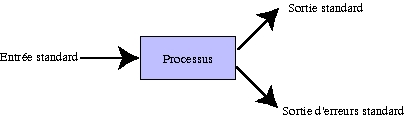
\includegraphics{base-concepts/iochans}
\caption{\label{fig-bcpts-iochans}Entr{\'e}es/Sorties d'un processus}
\end{figure}


Chacun des trois canaux se voit affecter un nom de fichier et un num{\'e}ro~:

\begin{tabular}{|l|c|c|}
	\hline
		\multicolumn{1}{|c|}{Canal de communication}		&
		\multicolumn{1}{|c|}{Fichier}						&
		\multicolumn{1}{|c|}{Num{\'e}ro logique}			\\
	\hline \hline
		Entr{\'e}e standard			&
		{\tt stdin}					&
		0							\\
	\hline
		Sortie standard				&
		{\tt stdout}				&
		1							\\
	\hline
		Sortie d'erreurs standard	&
		{\tt stderr}				&
		2							\\
	\hline
\end{tabular}

Le fichier \index{stdin@\texttt{stdin} (entr{\'e}e standard)}{\tt stdin} ({\sl entr{\'e}e standard}), est le fichier {\`a} partir duquel le process va lire les donn{\'e}es n{\'e}cessaires en entr{\'e}e. Il est ouvert avec le num{\'e}ro logique 0({\sl file descriptor C}), et il est, par d{\'e}faut associ{\'e} au clavier.

Le fichier \index{stdout@\texttt{stdout} (sortie standard)}{\tt stdout} ({\sl sortie standard}), est le fichier dans lequel le process va {\'e}crire les messages qu'il produit en sortie, dans le cas d'une ex{\'e}cution normale. Il est ouvert avec le num{\'e}ro logique 1 ({\sl file descriptor C}), et il est, par d{\'e}faut associ{\'e} {\`a} l'{\'e}cran.

Le fichier \index{stderr@\texttt{stderr} (sortie d'erreurs standard)}{\tt stderr} ({\sl sortie d'erreurs standard}), est le fichier dans lequel le process va {\'e}crire les messages d'erreur. Il est ouvert avec le num{\'e}ro logique 2 ({\sl file descriptor C}), et il est par d{\'e}faut associ{\'e} {\`a} l'{\'e}cran.

\begin{remarque}
On distingue toujours deux canaux de sorties (un pour les sorties normales et un pour les erreurs). En effet, si un process doit {\'e}crire dans un fichier et qu'une erreur se produit (impossibilit{\'e} d'{\'e}crire par exemple), il faut afficher un message sur un canal de sortie diff{\'e}rent.
\end{remarque}

Le tableau \ref{tab-bcpts-equiv-iochans} donne les {\'e}quivalences des noms
des canaux d'entr{\'e}es/sorties entre les syst{\`e}mes {\Unix} et {\OpenVMS} de Digital.

\begin{table}[hbtp]
\centering
\begin{tabular}{|l|c|c|}
	\hline
		{\Unix}	&	{\OpenVMS}	\\
	\hline \hline
		{\tt stdin}		&	\verb=SYS$INPUT=	\\
		{\tt stdout}	&	\verb=SYS$OUTPUT=	\\
		{\tt stderr}	&	\verb=SYS$ERROR=	\\
	\hline
\end{tabular}
\caption{\label{tab-bcpts-equiv-iochans}\'{E}quivalences des noms
des canaux d'entr{\'e}es/sorties entre {\Unix} et {\OpenVMS}}
\end{table}


%%%%%%%%%%%%%%%%%%%%%%%%%%%%%%%%%%%%%%%%%%%%%%%%%%%%%%%%%%%%%%%%%%%%%
\section{\label{bcpts-filters}Les filtres}

\index{filtre}Un filtre est une commande {\Unix} devant effectuer une action sur
les donn{\'e}es en lecture {\`a} partir de l'entr{\'e}e standard et afficher le
r{\'e}sultat en {\'e}criture sur la sortie standard.

La figure \ref{fig-bcpts-filters-desc} montre le principe des filtres sous
{\Unix}.

\begin{figure}[hbtp]
\centering
%\epsfbox{_Images/base-concepts/filters-desc.eps}
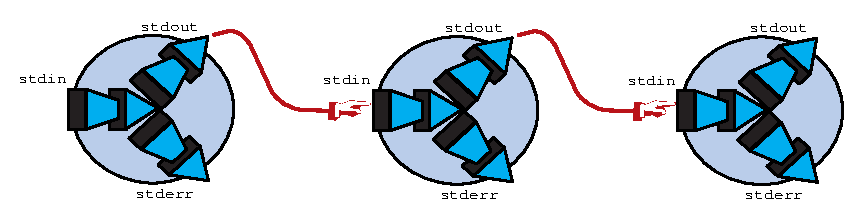
\includegraphics{base-concepts/filters-desc}
\caption{\label{fig-bcpts-filters-desc}Principe des filtres sous {\Unix}}
\end{figure}

Il est possible d'encha{\^\i}ner plusieurs filtres les uns aux autres. Par contre, les process en d{\'e}but et en fin de cha{\^\i}nes ne doivent pas se comporter comme des filtres.

